\documentclass[11pt, a4paper]{article}

% --- Core Packages ---
\usepackage[utf8]{inputenc}
\usepackage[T1]{fontenc}
\usepackage[libertine]{newtxmath}
\usepackage{libertine}
\usepackage[margin=1.1in]{geometry}
\usepackage{microtype}
\usepackage{authblk}
\usepackage{hyperref}
\usepackage{booktabs}
\usepackage{graphicx}
\usepackage{amsmath}
\usepackage{xcolor}
\usepackage{csquotes}
\usepackage[capitalize]{cleveref}
\usepackage{enumitem}
\usepackage{titlesec}
\usepackage[runin]{abstract}

% --- Aesthetics & Colors ---
\definecolor{navyblue}{RGB}{0,51,102}
\hypersetup{
    colorlinks=true,
    linkcolor=navyblue,
    citecolor=navyblue,
    urlcolor=navyblue,
    pdftitle={Sovereign Corpora: National Datasets for JoeyLLM},
}

% --- Section Styling ---
\titleformat{\section}{\large\bfseries\color{navyblue}}{\thesection}{1em}{}
\titleformat{\subsection}{\normalsize\bfseries\color{navyblue}}{\thesubsection}{1em}{}

% --- Abstract Styling ---
\renewcommand{\abstractnamefont}{\normalfont\small\bfseries\color{navyblue}}
\renewcommand{\abstracttextfont}{\normalfont\small}
\setlength{\absleftindent}{3em}
\setlength{\absrightindent}{3em}

% --- Custom Header ---
\makeatletter
\renewcommand{\maketitle}{
    \begin{center}
        {\LARGE\bfseries\color{navyblue} \@title \par}
        \vspace{1.5em}
        {\large \@author \par}
        \vspace{0.5em}
        {\small \textit{Southern Cross AI} \par}
        \vspace{0.8em}
        {\small \@date \par}
        \vspace{1.5em}
    \end{center}
}
\makeatother

\title{Sovereign Corpora: Extracting and Validating National Datasets for JoeyLLM}
\author{Matthew Altenburg}
\date{April 20, 2026}

\begin{document}

\maketitle

\begin{abstract}
Current large language models rely on web-scale datasets that lack cultural grounding, resulting in systems biased toward globally dominant distributions rather than region-specific contexts. While resources such as Common Crawl and curated derivatives like FineWeb provide high-quality large-scale corpora through extensive filtering and deduplication, they remain globally aggregated and are not structured to support the extraction of culturally coherent, national-level datasets. Furthermore, reproducing such pipelines from raw web data typically requires hyperscale infrastructure, limiting accessibility for most research groups.

In this work, we present a scalable and computationally efficient pipeline for constructing sovereign corpora by extending the FineWeb processing framework with targeted, domain-based extraction and structural refinement. Starting from Common Crawl via FineWeb, we apply ccTLD extraction and high-confidence structural refinement to isolate culturally grounded national subsets. Using the Australian context (\texttt{.au}) as a primary case study, we demonstrate the ability to extract and refine large-scale national datasets while maintaining broad topical coverage and internal coherence. We further validate the approach across multiple jurisdictions (\texttt{.uk}, \texttt{.ca}, \texttt{.nz}), confirming its general applicability.

To evaluate dataset quality, we employ embedding-based semantic projections and topic distribution analysis, demonstrating that the resulting corpora preserve diverse functional domains while exhibiting distinct regional characteristics. Our pipeline processes tens of terabytes of data in hours using modest GPU resources, enabling reproducible web-scale dataset construction without reliance on hyperscale infrastructure. These results establish a practical foundation for building culturally grounded datasets required for sovereign AI systems.
\end{abstract}

\section{Introduction}

Modern large language models are trained on massive web-scale datasets, often comprising trillions of tokens aggregated from diverse and heterogeneous sources. While these datasets enable broad linguistic coverage, they are typically dominated by globally prevalent content, particularly from a small number of high-volume regions. Consequently, the resulting models reflect a generalized, globalized distribution of language, often at the expense of region-specific linguistic patterns, cultural context, and local knowledge.

This lack of cultural grounding has significant practical implications. Language extends beyond vocabulary and spelling to include framing, institutional references, societal assumptions, and context-specific meaning. Models trained on globally mixed datasets frequently underrepresent or misinterpret these nuances, limiting their effectiveness in region-specific applications. As demand grows for AI systems aligned with national and institutional contexts, the need for datasets that accurately capture regional characteristics has become increasingly important.

Recent advances in dataset curation have focused on improving data quality at scale. Resources such as Common Crawl provide the foundational web corpus, while pipelines like FineWeb apply large-scale deduplication, language identification, and heuristic filtering to produce high-quality training data. These approaches have significantly improved the usability of web-scale datasets, but they remain globally aggregated and are not structured to support the extraction of culturally coherent, region-specific subsets.

At the same time, reproducing such large-scale filtering pipelines directly from raw web data typically requires hyperscale infrastructure. While large organizations can tokenize and index massive corpora for flexible downstream extraction, most research groups and institutions lack the computational resources to perform repeated full-scale processing of Common Crawl. This creates a practical barrier: although high-quality data exists, the ability to systematically derive targeted, culturally grounded datasets from it remains limited.

To address this gap, we present a scalable and computationally efficient pipeline for constructing national-level corpora by extending the FineWeb processing framework with targeted extraction and refinement stages. Starting from Common Crawl via FineWeb, our approach applies ccTLD extraction and structural refinement to isolate datasets that are statistically representative of specific national contexts. This pipeline is designed to operate under realistic computational constraints, enabling web-scale dataset construction without reliance on hyperscale infrastructure.

We validate the resulting datasets using embedding-based semantic analysis and distributional measurements, demonstrating that they retain broad topical coverage while exhibiting distinct regional characteristics. Furthermore, we show that this approach generalizes across multiple jurisdictions, providing a repeatable framework for constructing sovereign corpora. Together, these contributions establish a practical foundation for developing culturally grounded datasets required for sovereign AI systems.

\section{Background and Related Work}

The development of large-scale language models is closely tied to the availability of web-scale text corpora. Common Crawl serves as the primary foundation for such datasets, providing a continuously updated archive of publicly accessible web content. However, raw Common Crawl data is inherently noisy, containing significant amounts of boilerplate, duplication, and low-quality text, necessitating extensive filtering before it can be used for model training.

To address these challenges, recent work has focused on large-scale data curation pipelines. Approaches such as CCNet introduced systematic filtering techniques to improve data quality, while more recent efforts like FineWeb apply extensive deduplication, language identification, and heuristic scoring to produce high-quality, large-scale corpora suitable for modern pre-training. These pipelines represent a substantial advancement in making web-scale data usable, significantly reducing noise while preserving broad linguistic coverage.

Despite these improvements, existing pipelines are optimized for global data quality rather than geographic or cultural coherence. While language identification effectively separates content across languages, it does not capture regional variation within a shared language. As a result, datasets produced by these methods remain globally aggregated, masking the structural and contextual differences that define national or regional language use.

In parallel, there has been increasing interest in dataset transparency and analysis, including the use of topic modeling, metadata inspection, and embedding-based techniques to better understand corpus composition. While these approaches provide valuable insight into dataset characteristics, they are typically applied post hoc and do not directly support the construction of culturally grounded subsets at scale.

Efforts to build region-specific datasets have generally relied on manual curation or narrowly scoped data collection, which do not scale to the requirements of modern language model training. At the same time, reconstructing large-scale filtering pipelines directly from raw Common Crawl data remains computationally prohibitive for most research groups, requiring substantial infrastructure for repeated processing, deduplication, and tokenization.

This creates a fundamental gap between the availability of high-quality web-scale data and the ability to systematically derive targeted, culturally coherent corpora. While pipelines like FineWeb provide a high-quality global foundation, they do not enable efficient downstream extraction of region-specific datasets under realistic computational constraints. The method presented in this work addresses this gap by extending existing large-scale filtering frameworks with structured extraction and refinement techniques, enabling the construction of sovereign corpora without requiring hyperscale infrastructure.

\section{Data Pipeline Overview}

Our approach constructs sovereign corpora through a structured, multi-stage pipeline that progressively refines web-scale data into culturally grounded, region-specific datasets. The pipeline begins with Common Crawl, accessed via the FineWeb processing framework, which provides an initial layer of large-scale filtering including language identification, deduplication, and heuristic quality scoring. This stage produces a high-quality, globally aggregated English-language corpus that serves as the foundation for all subsequent processing.

The end-to-end dataflow for this process is summarized in \cref{fig:dataflow_pipeline}, while \cref{tab:pipeline_stages} defines the canonical stages used throughout this work.

\begin{figure}[ht]
    \centering
    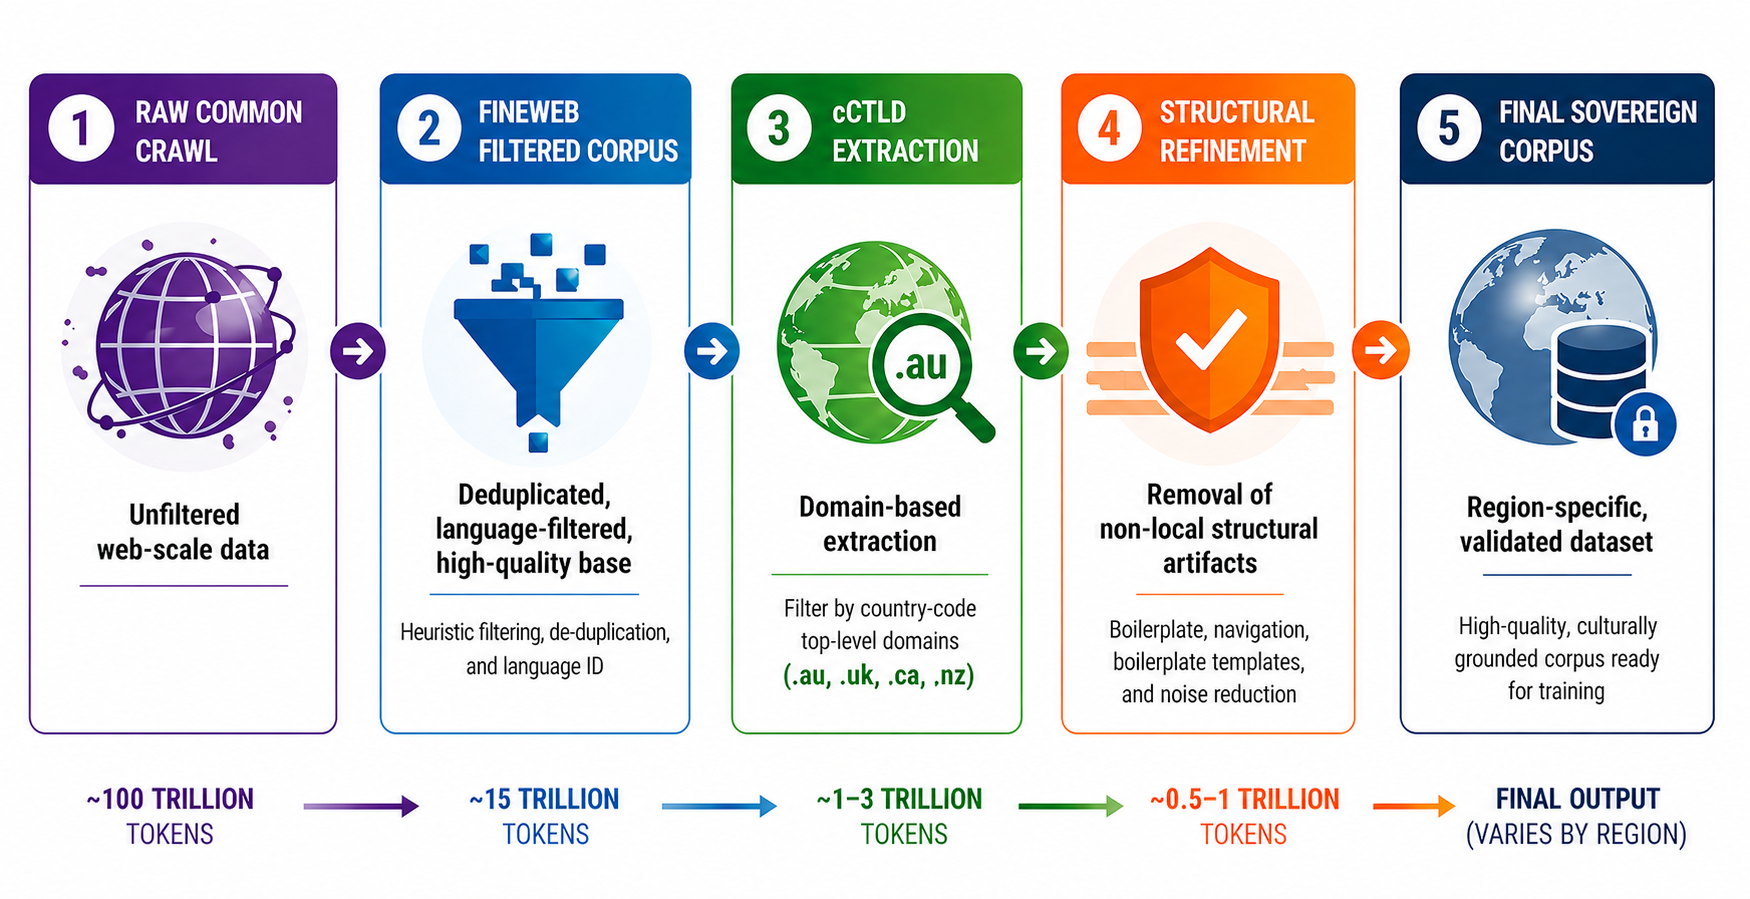
\includegraphics[width=\textwidth]{images/DataFlow.png}
    \caption{\textbf{Pipeline definition for sovereign corpus construction.} The dataflow illustrates the full processing path from Common Crawl and FineWeb ingestion through ccTLD extraction, structural refinement, dataset validation, and downstream sovereign corpus preparation.}
    \label{fig:dataflow_pipeline}
\end{figure}

\begin{table}[ht]
    \centering
    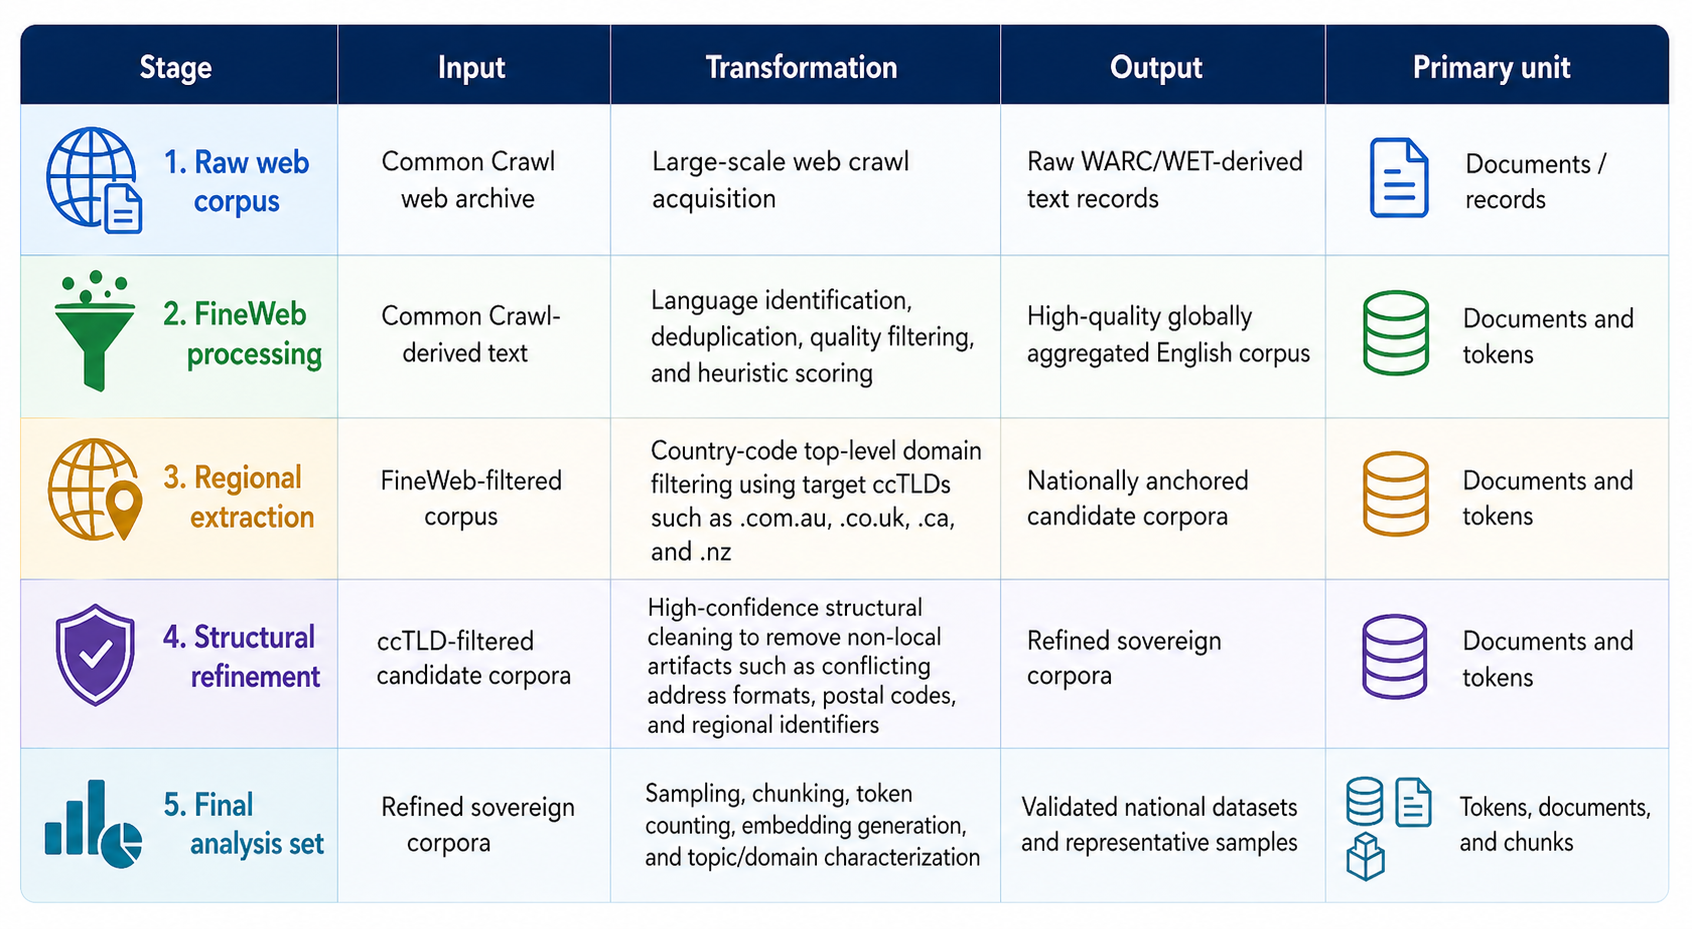
\includegraphics[width=\textwidth]{images/PipelineTable.png}
    \caption{\textbf{Canonical pipeline stages.} Summary of the data sources, processing stages, and outputs used throughout the sovereign corpus construction pipeline.}
    \label{tab:pipeline_stages}
\end{table}

\subsection{Pipeline Design and Philosophy}

The pipeline incorporates FineWeb as the global quality-filtering layer and adds targeted regional extraction and structural refinement stages. This distinction is important: the primary contribution of this work is not a replacement for FineWeb, but rather an extension of its web-scale curation into a practical framework for constructing sovereign corpora under realistic computational constraints.

\subsection{Tokenization and Measurement}

Token counts reported in this paper are derived from the \texttt{token\_count} field provided in the FineWeb dataset metadata. FineWeb defines this field as the number of tokens obtained by applying the GPT-2 tokenizer to each document's text column. We do not retokenize documents in our pipeline; instead, corpus-level token totals are calculated by summing FineWeb's existing \texttt{token\_count} values across retained documents after ccTLD extraction and structural refinement. This ensures consistency with the source corpus while allowing token volumes to be tracked across downstream stages. Future iterations that reprocess Common Crawl directly will explicitly define the tokenizer used at the raw-processing stage.

We distinguish between three primary units of measure:

\begin{itemize}[noitemsep]
    \item \textbf{Documents:} A single FineWeb record, corresponding to one row containing text, URL, metadata, and language score.
    \item \textbf{Tokens:} The upstream token count associated with each document, used to estimate corpus scale.
    \item \textbf{Chunks:} Smaller text segments derived from documents for downstream sampling, embedding generation, and semantic analysis.
\end{itemize}

Unless otherwise stated, extraction statistics are reported at the document and token level, while validation statistics are reported at the chunk level.

\subsection{Storage and Scale}

Storage volumes are reported using compressed source size unless otherwise specified. Because the source data is stored in compressed Parquet format, decompressed in-memory size varies based on text length, metadata density, and compression ratios. Therefore, compressed byte counts serve as our primary reproducible storage measure, as summarized in \cref{tab:data_size_conventions}. We do not report uncompressed corpus size as a primary metric because decompressed size depends on Parquet decoding, selected columns, metadata expansion, and runtime representation.

\begin{table}[ht]
    \centering
    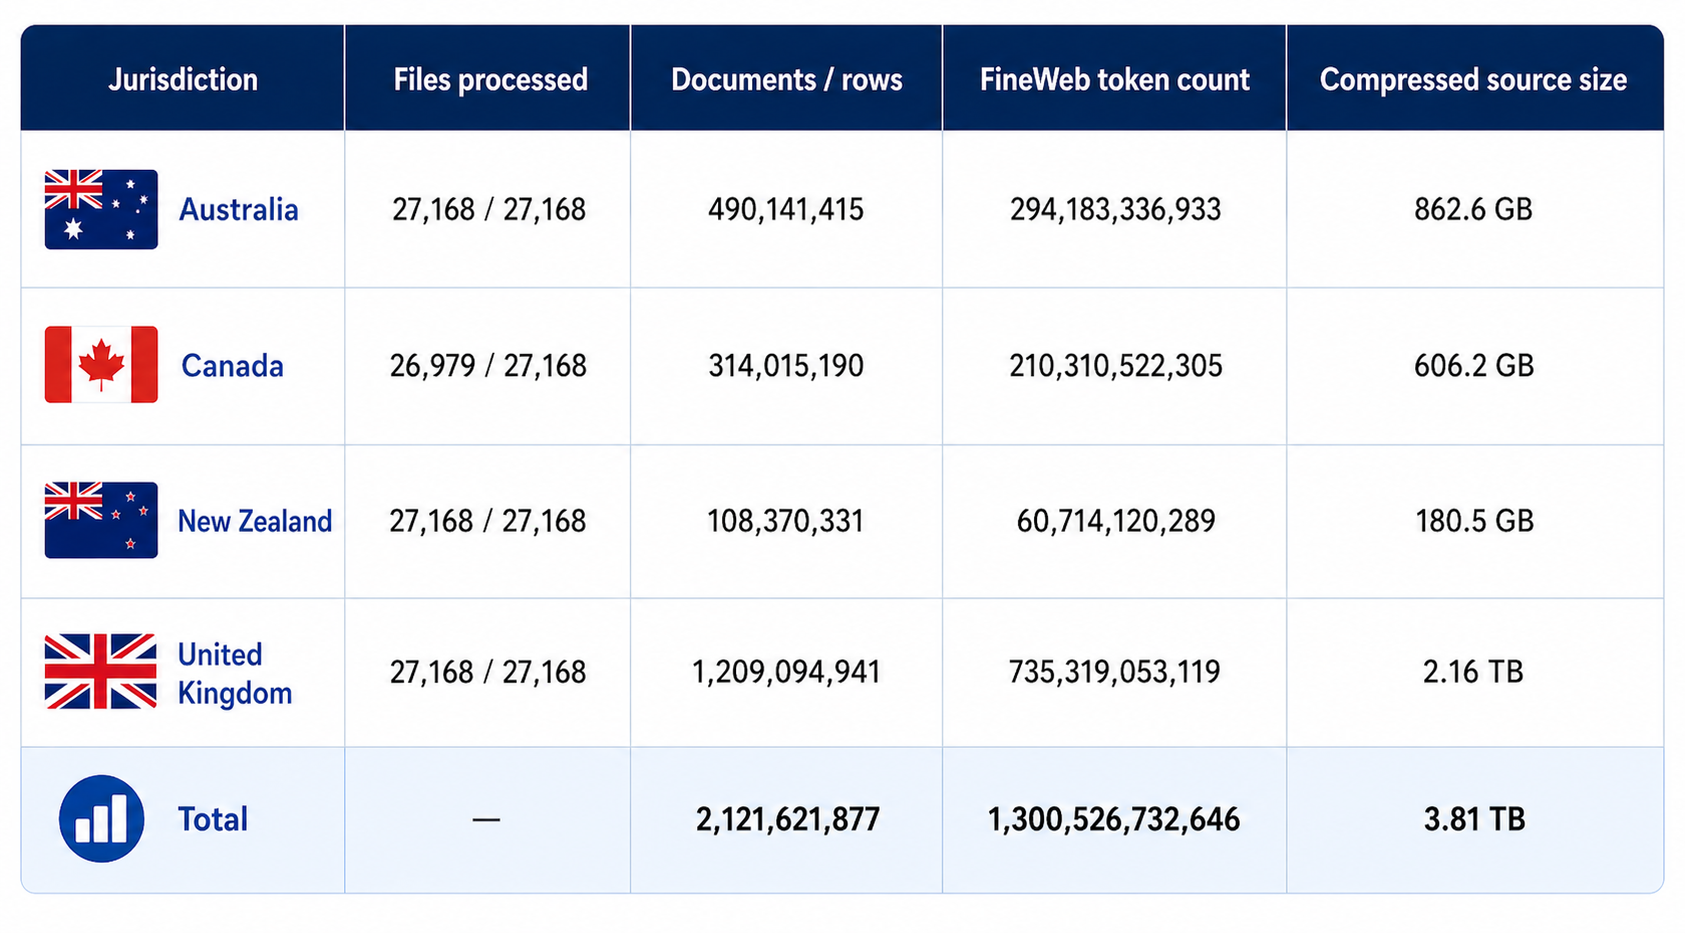
\includegraphics[width=\textwidth]{images/DataSize.png}
    \caption{\textbf{Data size conventions.} Summary of storage, retained source data, and token-volume reporting used throughout the pipeline.}
    \label{tab:data_size_conventions}
\end{table}

In this work:

\begin{itemize}[noitemsep]
    \item \textbf{60TB} refers to the total FineWeb input corpus scanned.
    \item \textbf{3.81TB} refers to the compressed retained source data across Australia, the United Kingdom, Canada, and New Zealand following ccTLD extraction.
    \item \textbf{1.3 trillion tokens} refers to the summed FineWeb \texttt{token\_count} values across retained documents.
\end{itemize}

\subsection{Fault Tolerance and Extraction}

The pipeline is fault-tolerant at the file level; corrupted or unreadable files are skipped rather than terminating the run. Reported file counts reflect successfully processed source files. For example, in the Canadian extraction, 26,979 of 27,168 source files were successfully processed, with the remainder excluded due to read or corruption errors.

\subsection{Regional Refinement}

We introduce targeted extraction stages designed to isolate culturally coherent subsets:

\begin{itemize}[noitemsep]
    \item \textbf{ccTLD extraction:} Country-code top-level domains, such as \texttt{.au}, \texttt{.uk}, \texttt{.ca}, and \texttt{.nz}, are used as high-confidence proxies for regional origin. This shifts the distribution from a globally mixed corpus toward geographically anchored subsets.
    \item \textbf{Structural refinement:} A secondary stage removes residual non-local artifacts using structural signals, such as conflicting address formats or postal codes, rather than semantic content. The objective is to improve internal consistency while preserving legitimate cross-regional discourse.
\end{itemize}

\subsection{Computational Implementation}

The pipeline is designed for efficiency in non-hyperscale environments. By leveraging GPU-accelerated frameworks including \texttt{cuDF}, \texttt{Dask}, and \texttt{PyArrow}, the system processes parallelized batches of compressed content. This architecture enables high-throughput ingestion and transformation using a modest number of GPUs, ensuring the framework remains accessible for specialized sovereign research.

\section{Country-Level Dataset Extraction}

To derive national-level corpora from the globally aggregated FineWeb dataset, we employ country-code top-level domain (ccTLD) filtering as the primary mechanism for approximating geographic and cultural origin. While web-scale data is inherently global and unbounded, domains such as \texttt{.au}, \texttt{.uk}, \texttt{.ca}, and \texttt{.nz} provide a scalable and high-confidence signal of regional affiliation. These domains are predominantly associated with domestic institutions, including government agencies, local media, educational organizations, and regional businesses, making them effective proxies for culturally grounded content.

The extraction process systematically isolates all documents matching the target ccTLD patterns from the FineWeb-filtered corpus. This produces large-scale subsets that significantly shift the underlying data distribution away from global aggregation toward regionally concentrated datasets. At scale, this approach yields hundreds of billions of tokens per jurisdiction, reflecting the relative digital footprint of each country while maintaining sufficient volume for downstream model training and analysis.

We acknowledge that ccTLD extraction is an imperfect proxy for geographic origin. Multinational organizations may host content on country-specific domains, while substantial volumes of domestic content may reside on generic domains such as \texttt{.com} or \texttt{.org}. However, at web-scale, these effects are statistically dominated by the primary signal, allowing ccTLD extraction to produce datasets with strong regional characteristics despite localized noise.

Importantly, this extraction method is applied consistently across all target jurisdictions. By maintaining identical filtering criteria and processing logic, we ensure that observed differences between national datasets reflect genuine variation in underlying web content rather than inconsistencies in methodology. This consistency is critical for both comparative analysis and downstream applications, where relative differences between datasets carry interpretive significance.

The resulting corpora form the foundation for subsequent refinement stages, where additional structural refinement is applied to further improve dataset coherence and alignment. Through this approach, we establish a scalable and repeatable method for isolating high-confidence national datasets from globally mixed web-scale sources.

\section{Data Cleaning and Filtering}

Following ccTLD extraction, we apply a secondary structural refinement stage to improve dataset coherence and remove residual non-local artifacts. While ccTLD extraction provides a strong geographic prior, it does not fully eliminate misaligned content, as globally distributed material and templated web structures can persist within regionally scoped domains.

To address these limitations, we introduce a structural refinement stage that operates independently of semantic content. Rather than evaluating topic or meaning, this stage targets high-confidence structural indicators of geographic inconsistency, such as conflicting address formats, postal codes, and standardized regional identifiers that do not align with the target jurisdiction. By focusing on structural signals, the pipeline avoids overfitting to topical content and preserves legitimate cross-regional discourse embedded within local sources.

This design ensures that content reflecting international events or entities is retained when framed within a domestic context, while only text that exhibits clear structural evidence of external origin is removed. As a result, the refinement process improves internal consistency without artificially narrowing the topical scope of the dataset.

In practice, this structural refinement stage removes a relatively small proportion of the total extracted tokens. This outcome serves as an implicit validation of the ccTLD extraction step, indicating that the majority of the data already aligns with the intended regional signal. The process therefore acts as a refinement layer rather than a primary filter, correcting edge cases and reinforcing dataset integrity.

The combination of ccTLD extraction and structural refinement yields datasets that are both statistically representative and internally coherent. These refined corpora are then passed to downstream validation stages to assess their semantic structure and suitability for sovereign AI applications.

\section{Dataset Characterization}

Following extraction and structural refinement, we characterize the composition, diversity, and semantic structure of the resulting datasets. Given the scale of these corpora, direct inspection is infeasible; therefore, we rely on statistical sampling and embedding-based analysis to evaluate their internal properties.

To assess topical coverage, we generate vector embeddings for a representative sample of each national dataset. These embeddings are compared against a predefined set of semantic anchors corresponding to broad functional domains, such as government, media, education, business, and science. Each sampled text segment is assigned to its nearest semantic anchor, allowing us to construct a high-level distribution of content across these domains.

This analysis provides a coarse but effective measure of whether the extraction and filtering pipeline preserves broad topical diversity or collapses into a narrow subset of high-frequency content. Across all evaluated datasets, we observe a balanced distribution of topics, indicating that the pipeline maintains coverage across multiple functional domains rather than overrepresenting a small number of sources.

\begin{figure}[ht]
    \centering
    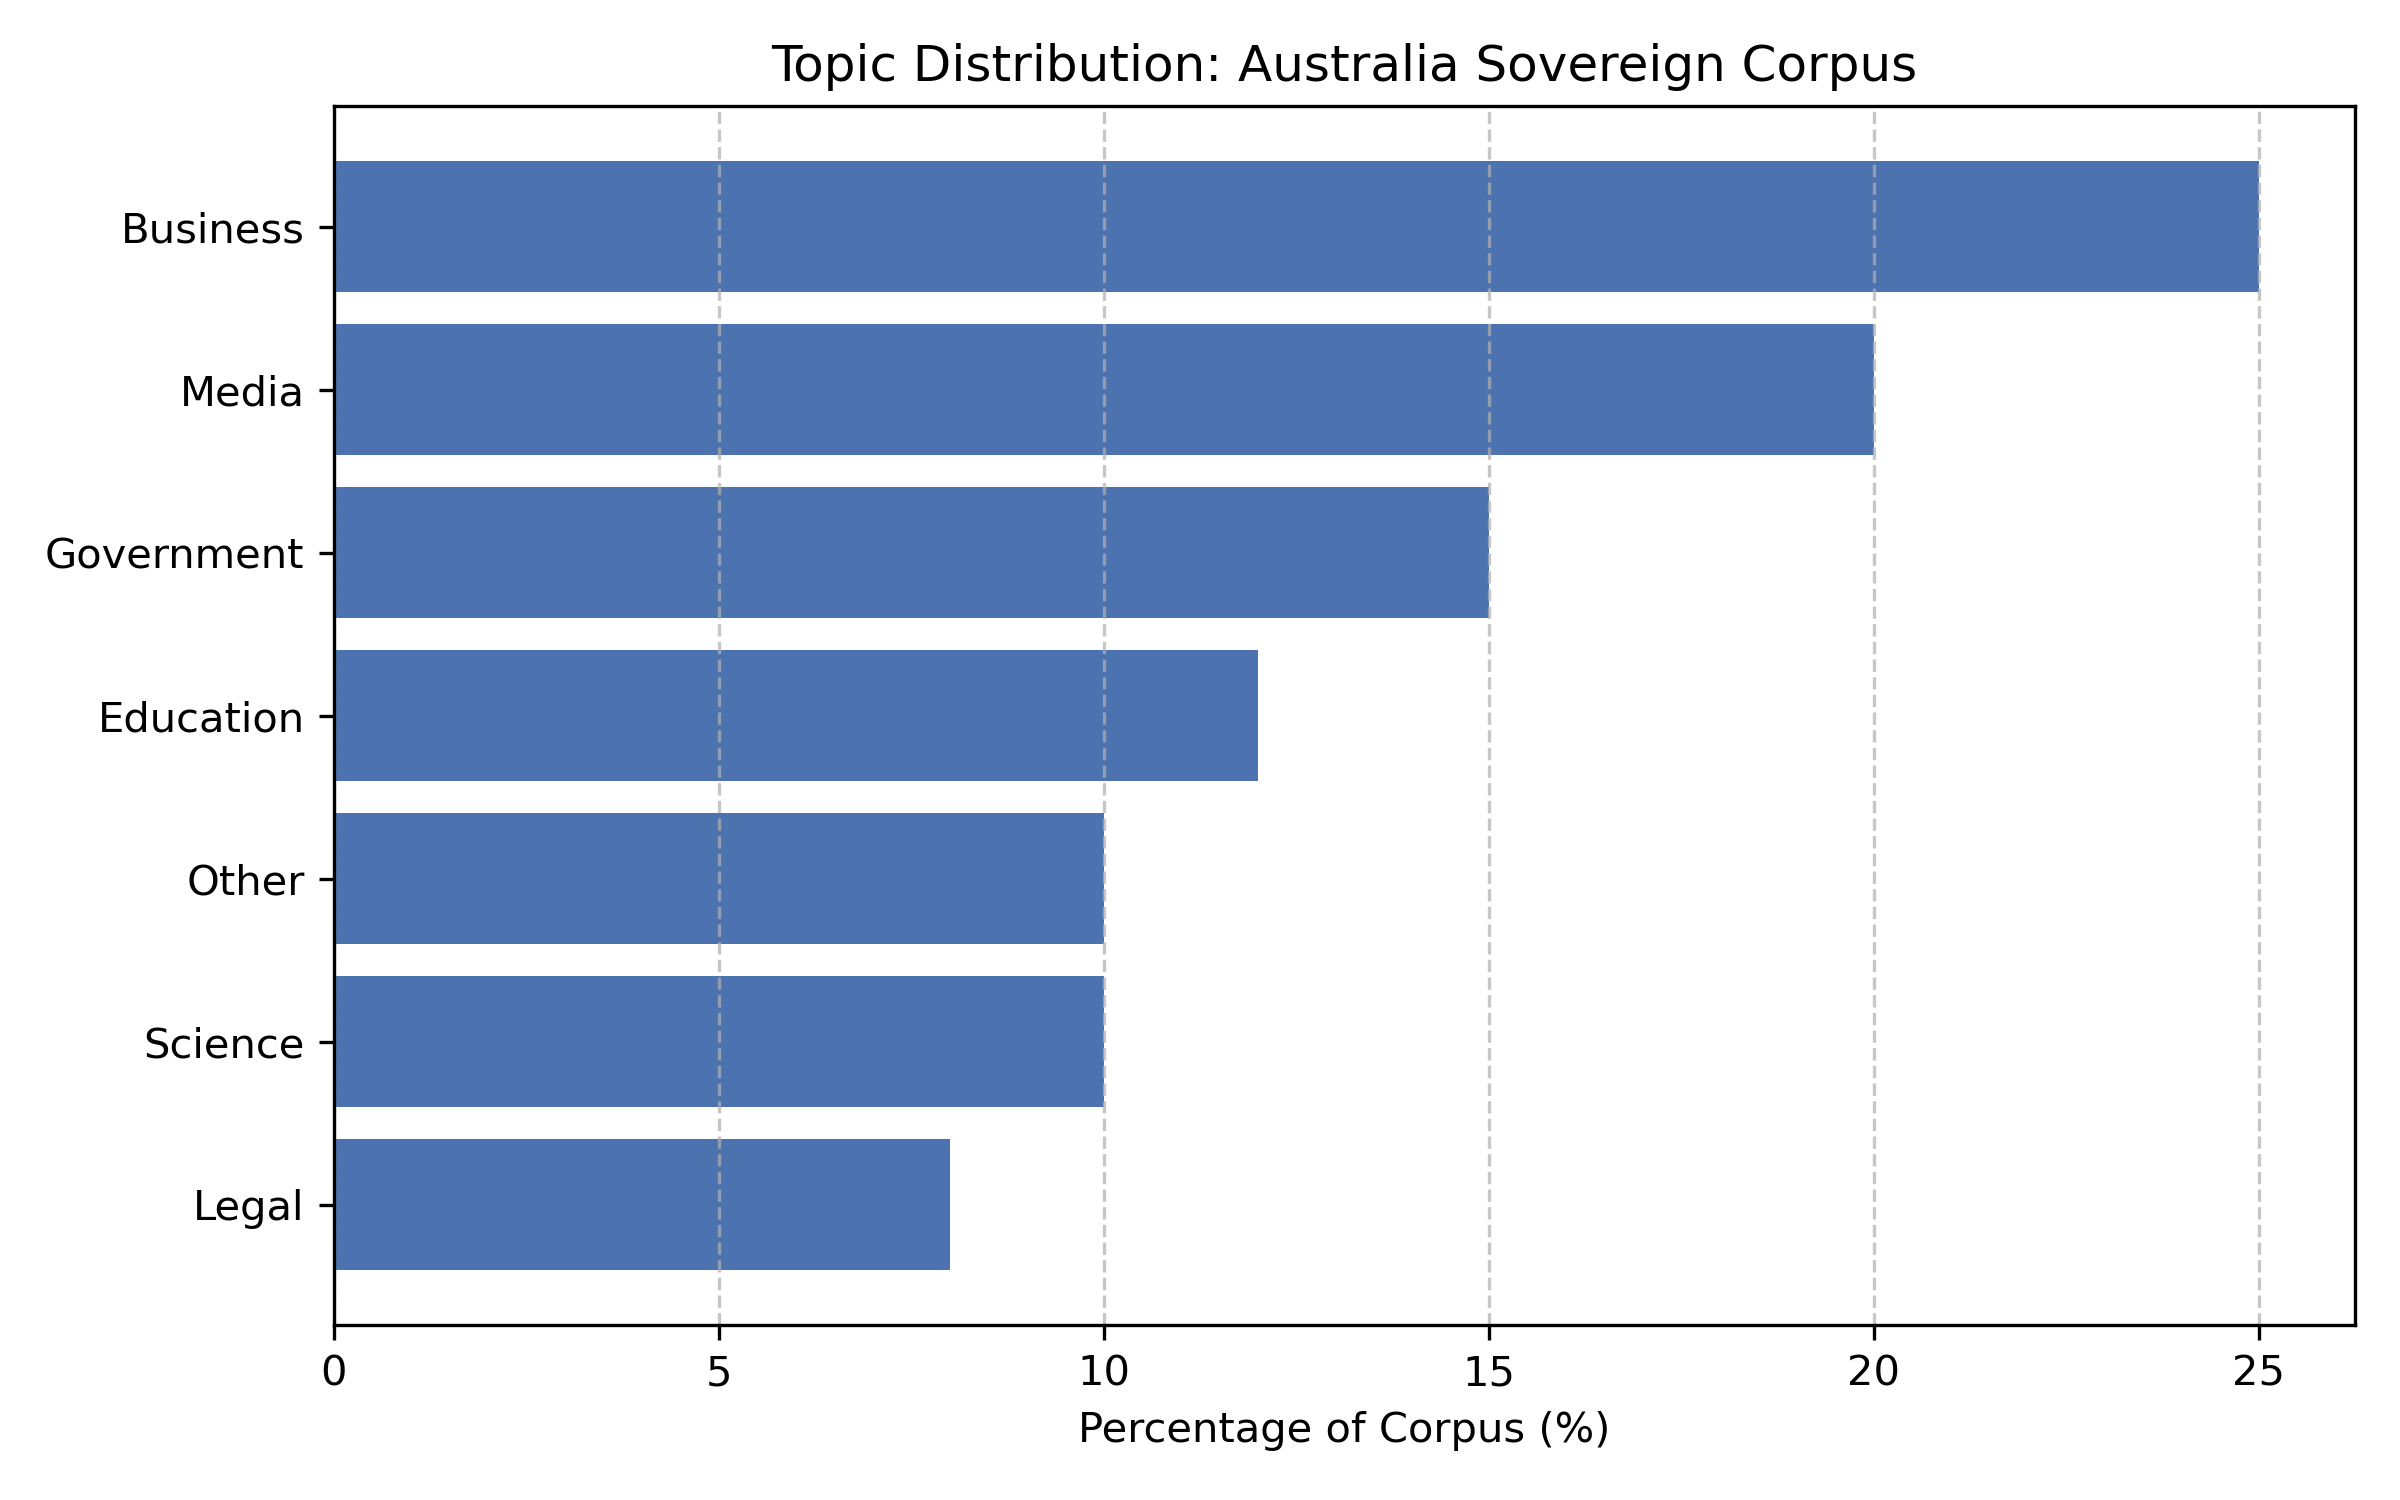
\includegraphics[width=0.85\textwidth]{images/fig2.png}
    \caption{Topic Distribution: Australia Sovereign Corpus. The proportion of sampled chunks assigned to broad functional domains.}
    \label{fig:topic_dist_au}
\end{figure}

In addition to topic distribution, we examine the structural coherence of the datasets within the embedding space. By projecting embeddings into lower-dimensional representations, we observe the formation of dense, well-defined clusters corresponding to distinct semantic groupings. These clusters indicate that the datasets retain meaningful internal organization, rather than exhibiting fragmented or noisy distributions.

\begin{figure}[ht]
    \centering
    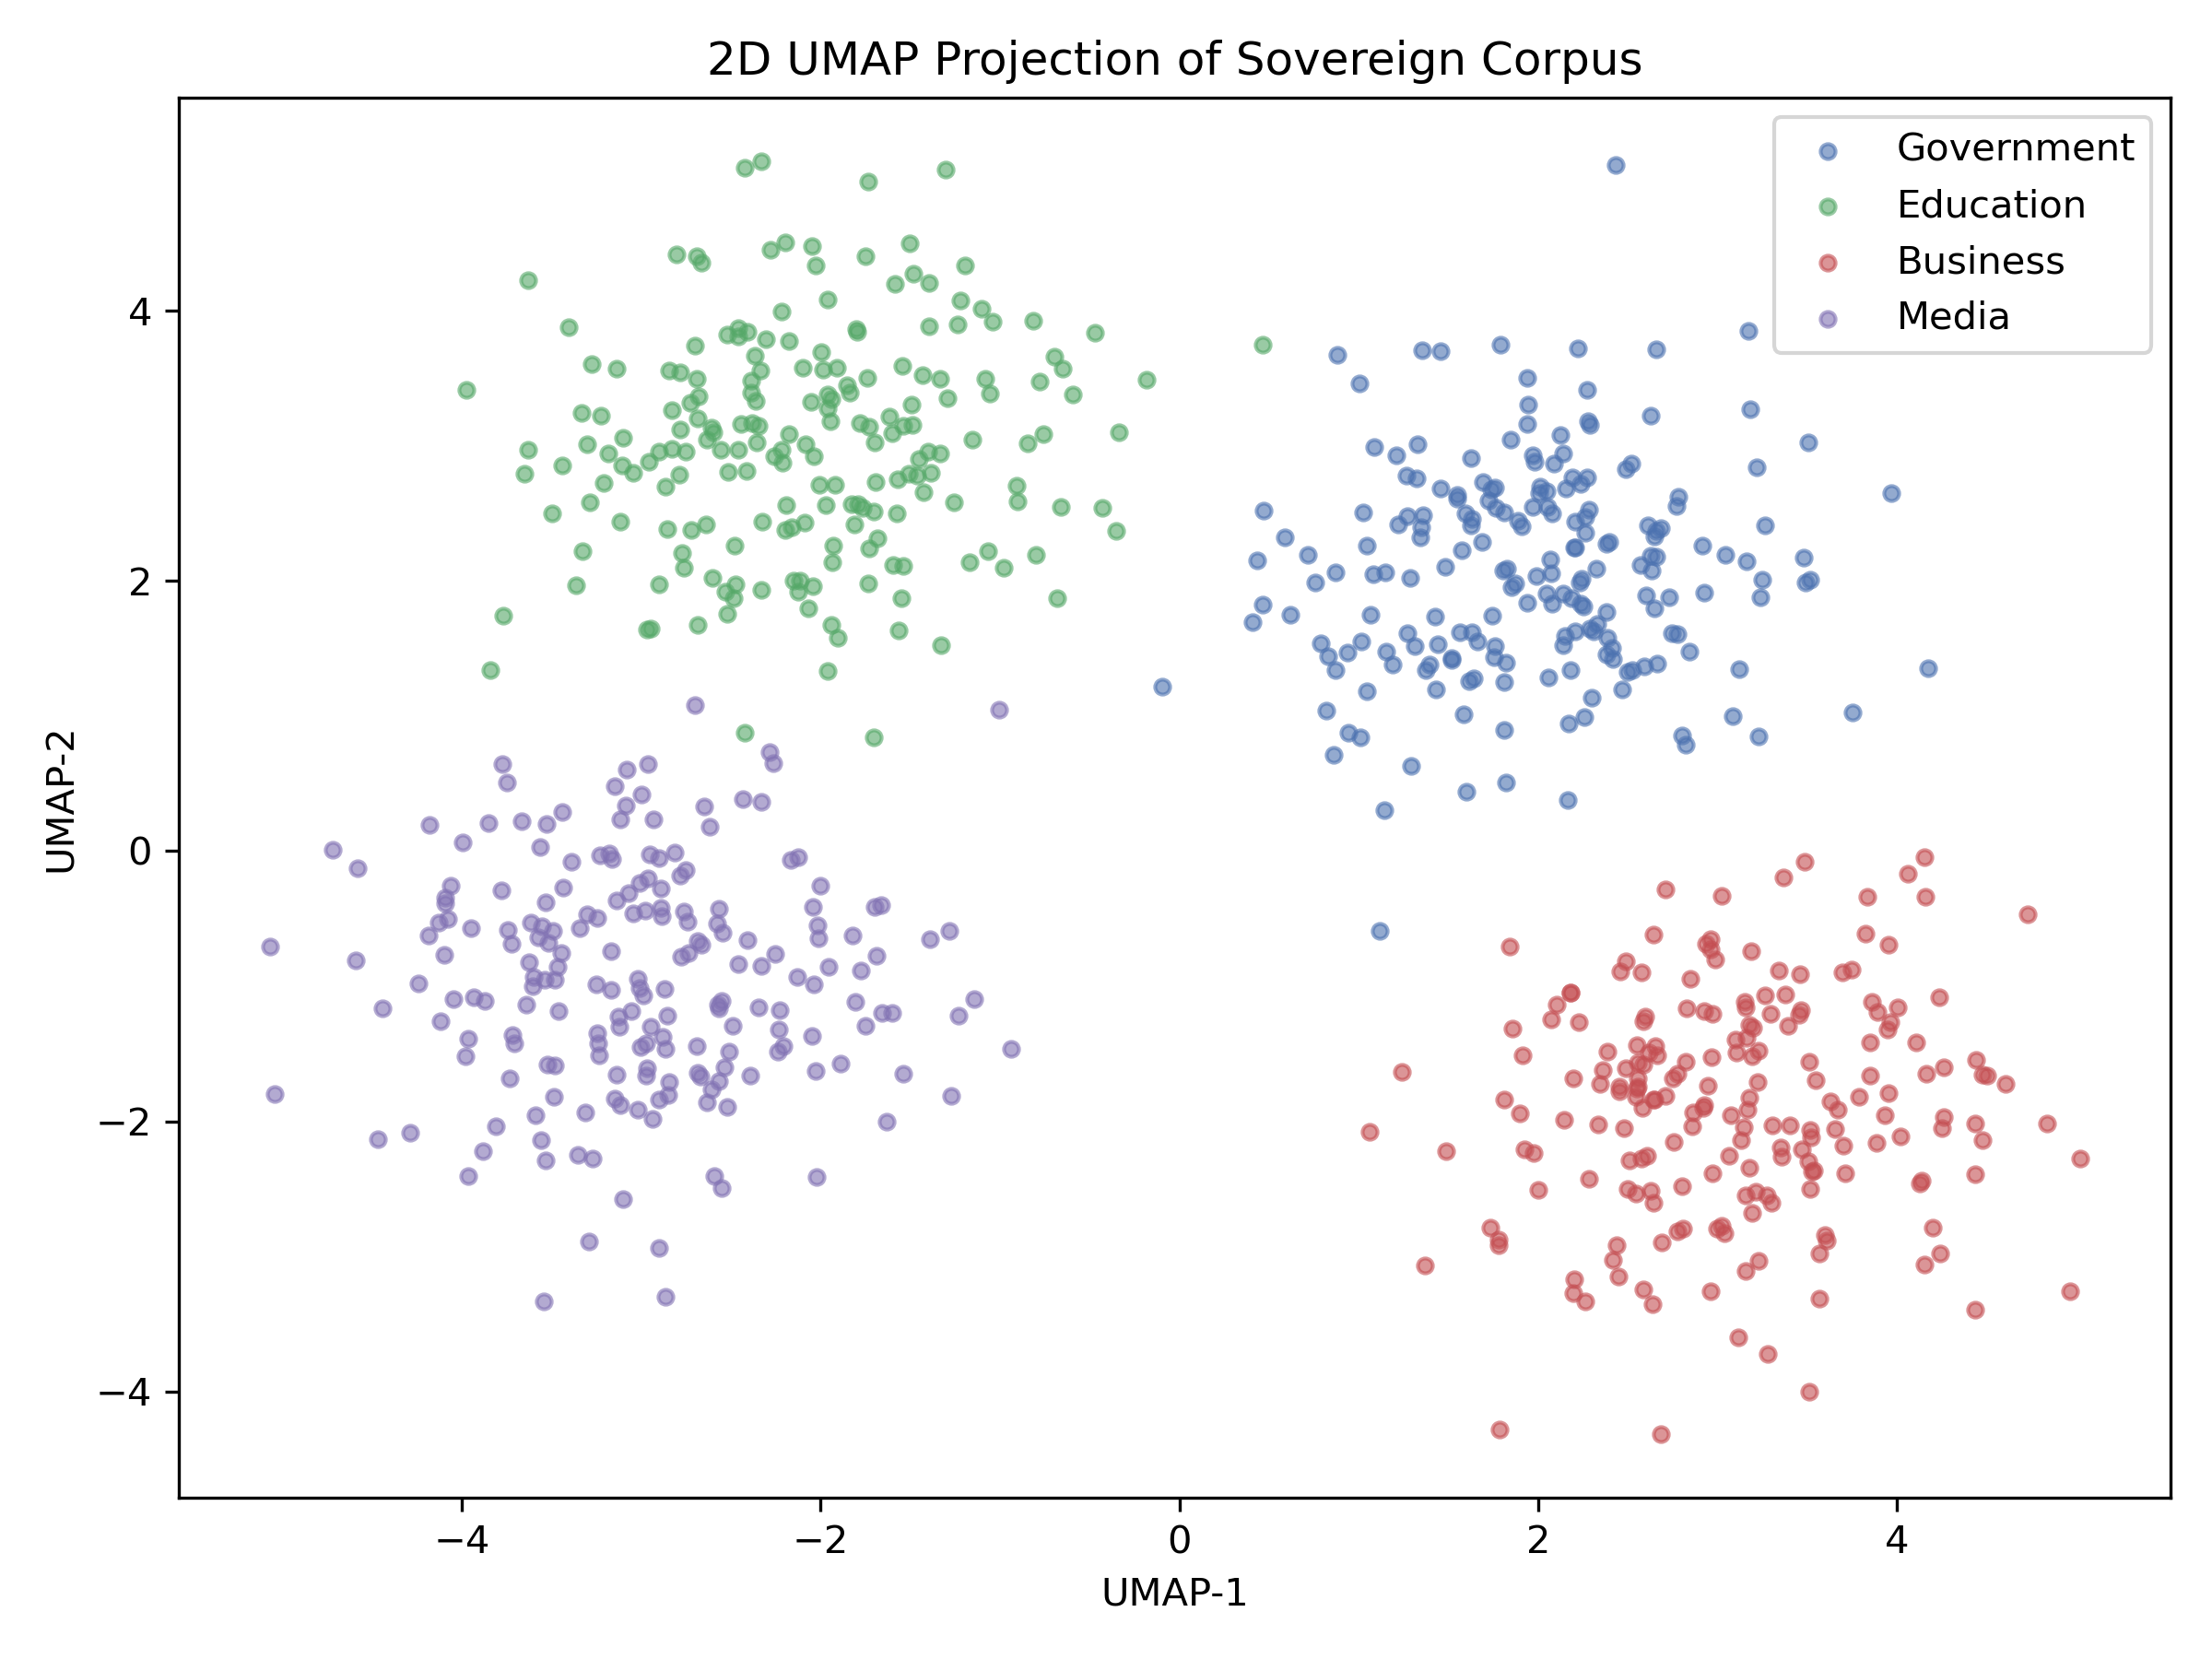
\includegraphics[width=0.85\textwidth]{images/fig3.png}
    \caption{Semantic Projection of a Sovereign Corpus. 2D UMAP visualization of text embeddings, color-coded by topic, illustrating the coherent internal structure of the extracted data.}
    \label{fig:umap_projection}
\end{figure}

Together, these characterization methods provide evidence that the pipeline produces datasets that are both diverse and structurally coherent. This validation step is critical in demonstrating that the extraction process preserves the richness of the original web data while successfully shifting the distribution toward culturally grounded, region-specific content.

\section{Cross-Country Comparison}

To evaluate the generalizability of the extraction pipeline, we apply the same ccTLD extraction and structural refinement process across multiple jurisdictions, including Australia, the United Kingdom, Canada, and New Zealand. Because each dataset is derived from the same underlying FineWeb corpus and processed using identical pipeline stages, any observed differences reflect genuine variation in regional web content rather than inconsistencies in methodology.

Across all jurisdictions, the resulting datasets maintain large scale, broad topical coverage, and strong internal coherence. This consistency demonstrates that the pipeline is not dependent on region-specific tuning, but instead operates as a generalizable framework for extracting culturally grounded corpora from globally aggregated data.

Despite these shared high-level properties, meaningful differences emerge in the composition of each national dataset. Topic distributions vary across countries, reflecting differences in institutional presence, media ecosystems, and commercial activity. For example, some datasets exhibit higher representation of government and educational content, while others are more heavily weighted toward commercial or media domains. These variations indicate that the extraction process preserves underlying structural characteristics of each region rather than producing uniform subsets.

\begin{figure}[ht]
    \centering
    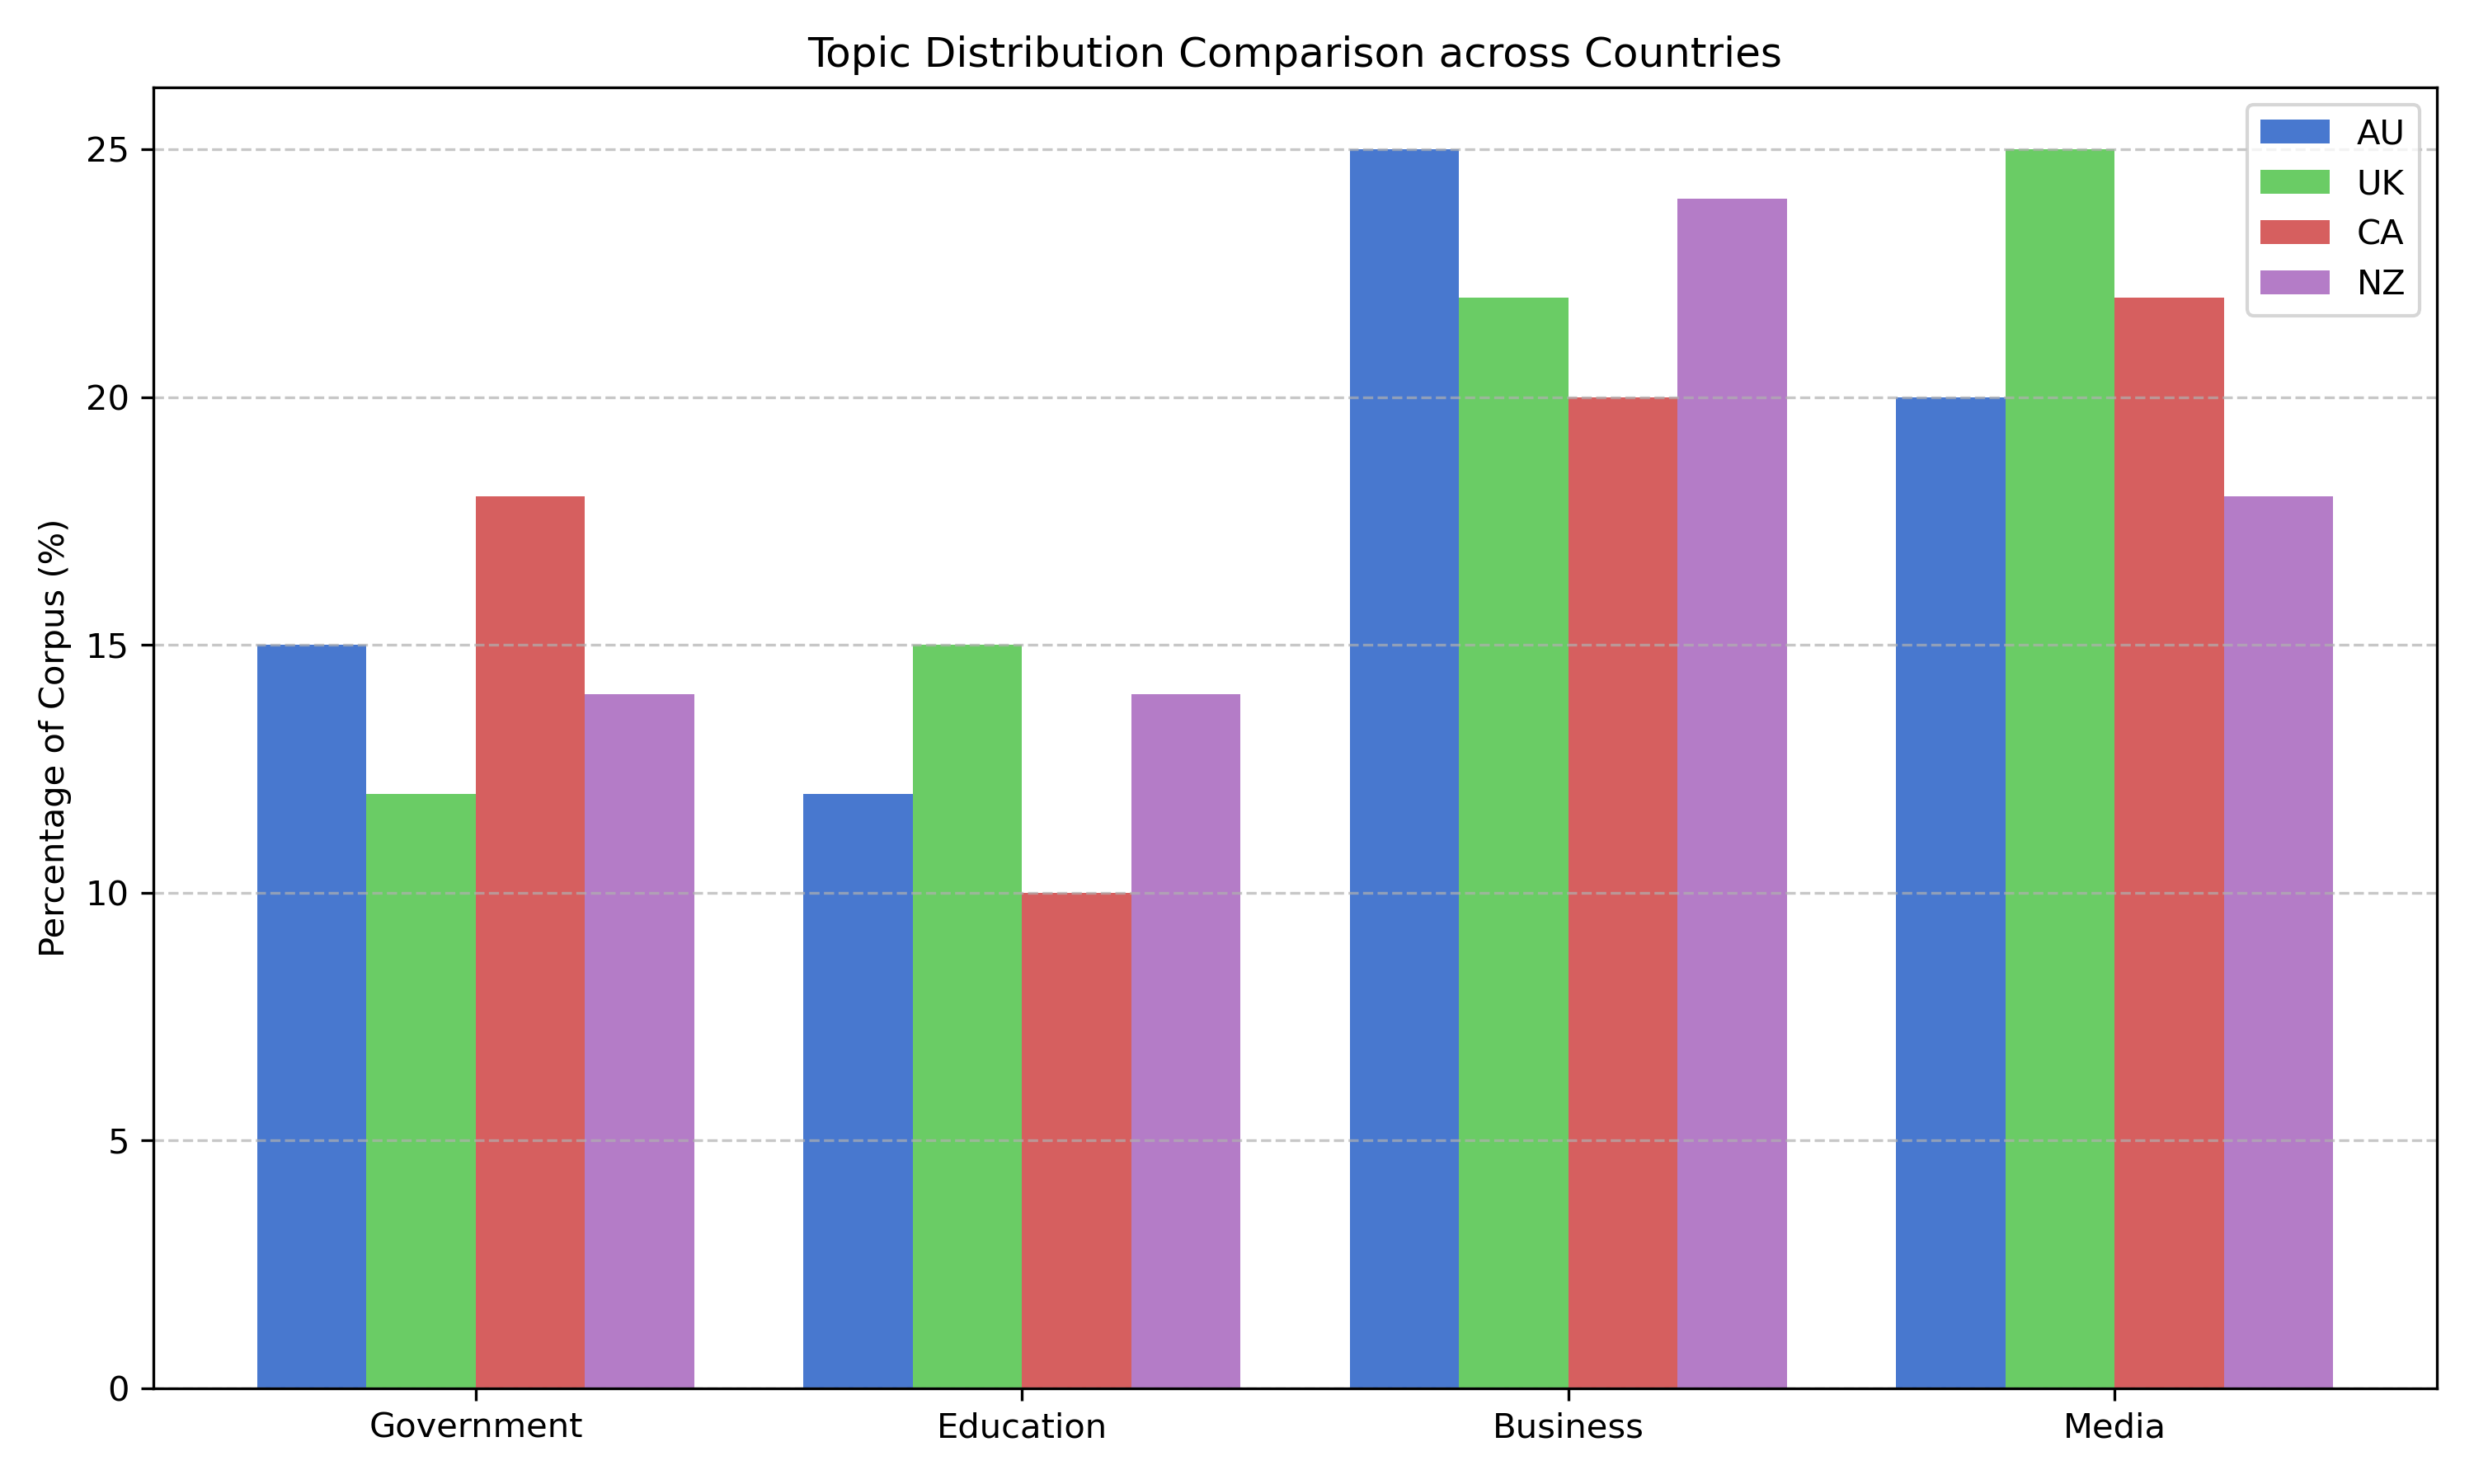
\includegraphics[width=0.85\textwidth]{images/fig4.png}
    \caption{Topic Distribution Comparison across Countries. Grouped bar chart comparing topic proportions across AU, UK, CA, and NZ, highlighting meaningful regional variance.}
    \label{fig:topic_dist_cross}
\end{figure}

Further analysis using embedding-based projections reinforces these findings. When visualized in a shared semantic space, each national corpus forms coherent internal clusters while also exhibiting measurable divergence from other countries. Equivalent semantic groupings---such as media or government content---show subtle shifts in distribution, reflecting differences in terminology, institutional structures, and contextual framing across regions.

These results confirm that the pipeline captures region-specific characteristics at scale, producing datasets that are not only internally coherent but also meaningfully distinct from one another. This cross-country consistency and divergence provide strong evidence that the method is suitable for constructing sovereign corpora across diverse national contexts.

\section{Domain Substructure within National Corpora}

Beyond country-level extraction, we examine whether the resulting national datasets exhibit meaningful internal structure that can be further decomposed into functional sub-corpora. Specifically, we evaluate whether domains such as government, education, media, and commercial activity form identifiable and coherent subsets within the broader national corpus.

To assess this, we apply embedding-based semantic analysis at a finer level of granularity. Representative samples from each national dataset are projected against domain-specific semantic anchors, enabling the identification of dense regions in the embedding space corresponding to distinct functional categories. This approach allows us to determine whether the datasets retain structured internal organization or collapse into indistinguishable semantic distributions.

Our analysis indicates that the extracted corpora can be consistently decomposed into well-defined substructures. Within each national dataset, distinct clusters emerge that align with major functional domains, demonstrating that the pipeline preserves not only high-level topical diversity but also fine-grained semantic organization. These clusters are not diffuse or overlapping, but instead form coherent conceptual groupings that reflect underlying real-world data distributions.

Importantly, the relative proportions of these sub-corpora vary across jurisdictions, reinforcing earlier observations from cross-country comparisons. Differences in the representation of government, educational, media, and commercial content reflect genuine variation in national web ecosystems rather than artifacts of the extraction process.

This internal structure has practical implications. The ability to isolate coherent domain-specific subsets from within a national corpus suggests that the pipeline can support more targeted dataset construction without requiring additional large-scale data collection. As a result, the extracted datasets are not only suitable for broad sovereign AI training, but also adaptable to more specialized applications that require focused, high-confidence data subsets.

Overall, this analysis provides a final layer of validation, demonstrating that the pipeline produces datasets that are both structurally coherent at the national level and internally decomposable into meaningful functional domains.

\begin{figure}[ht]
    \centering
    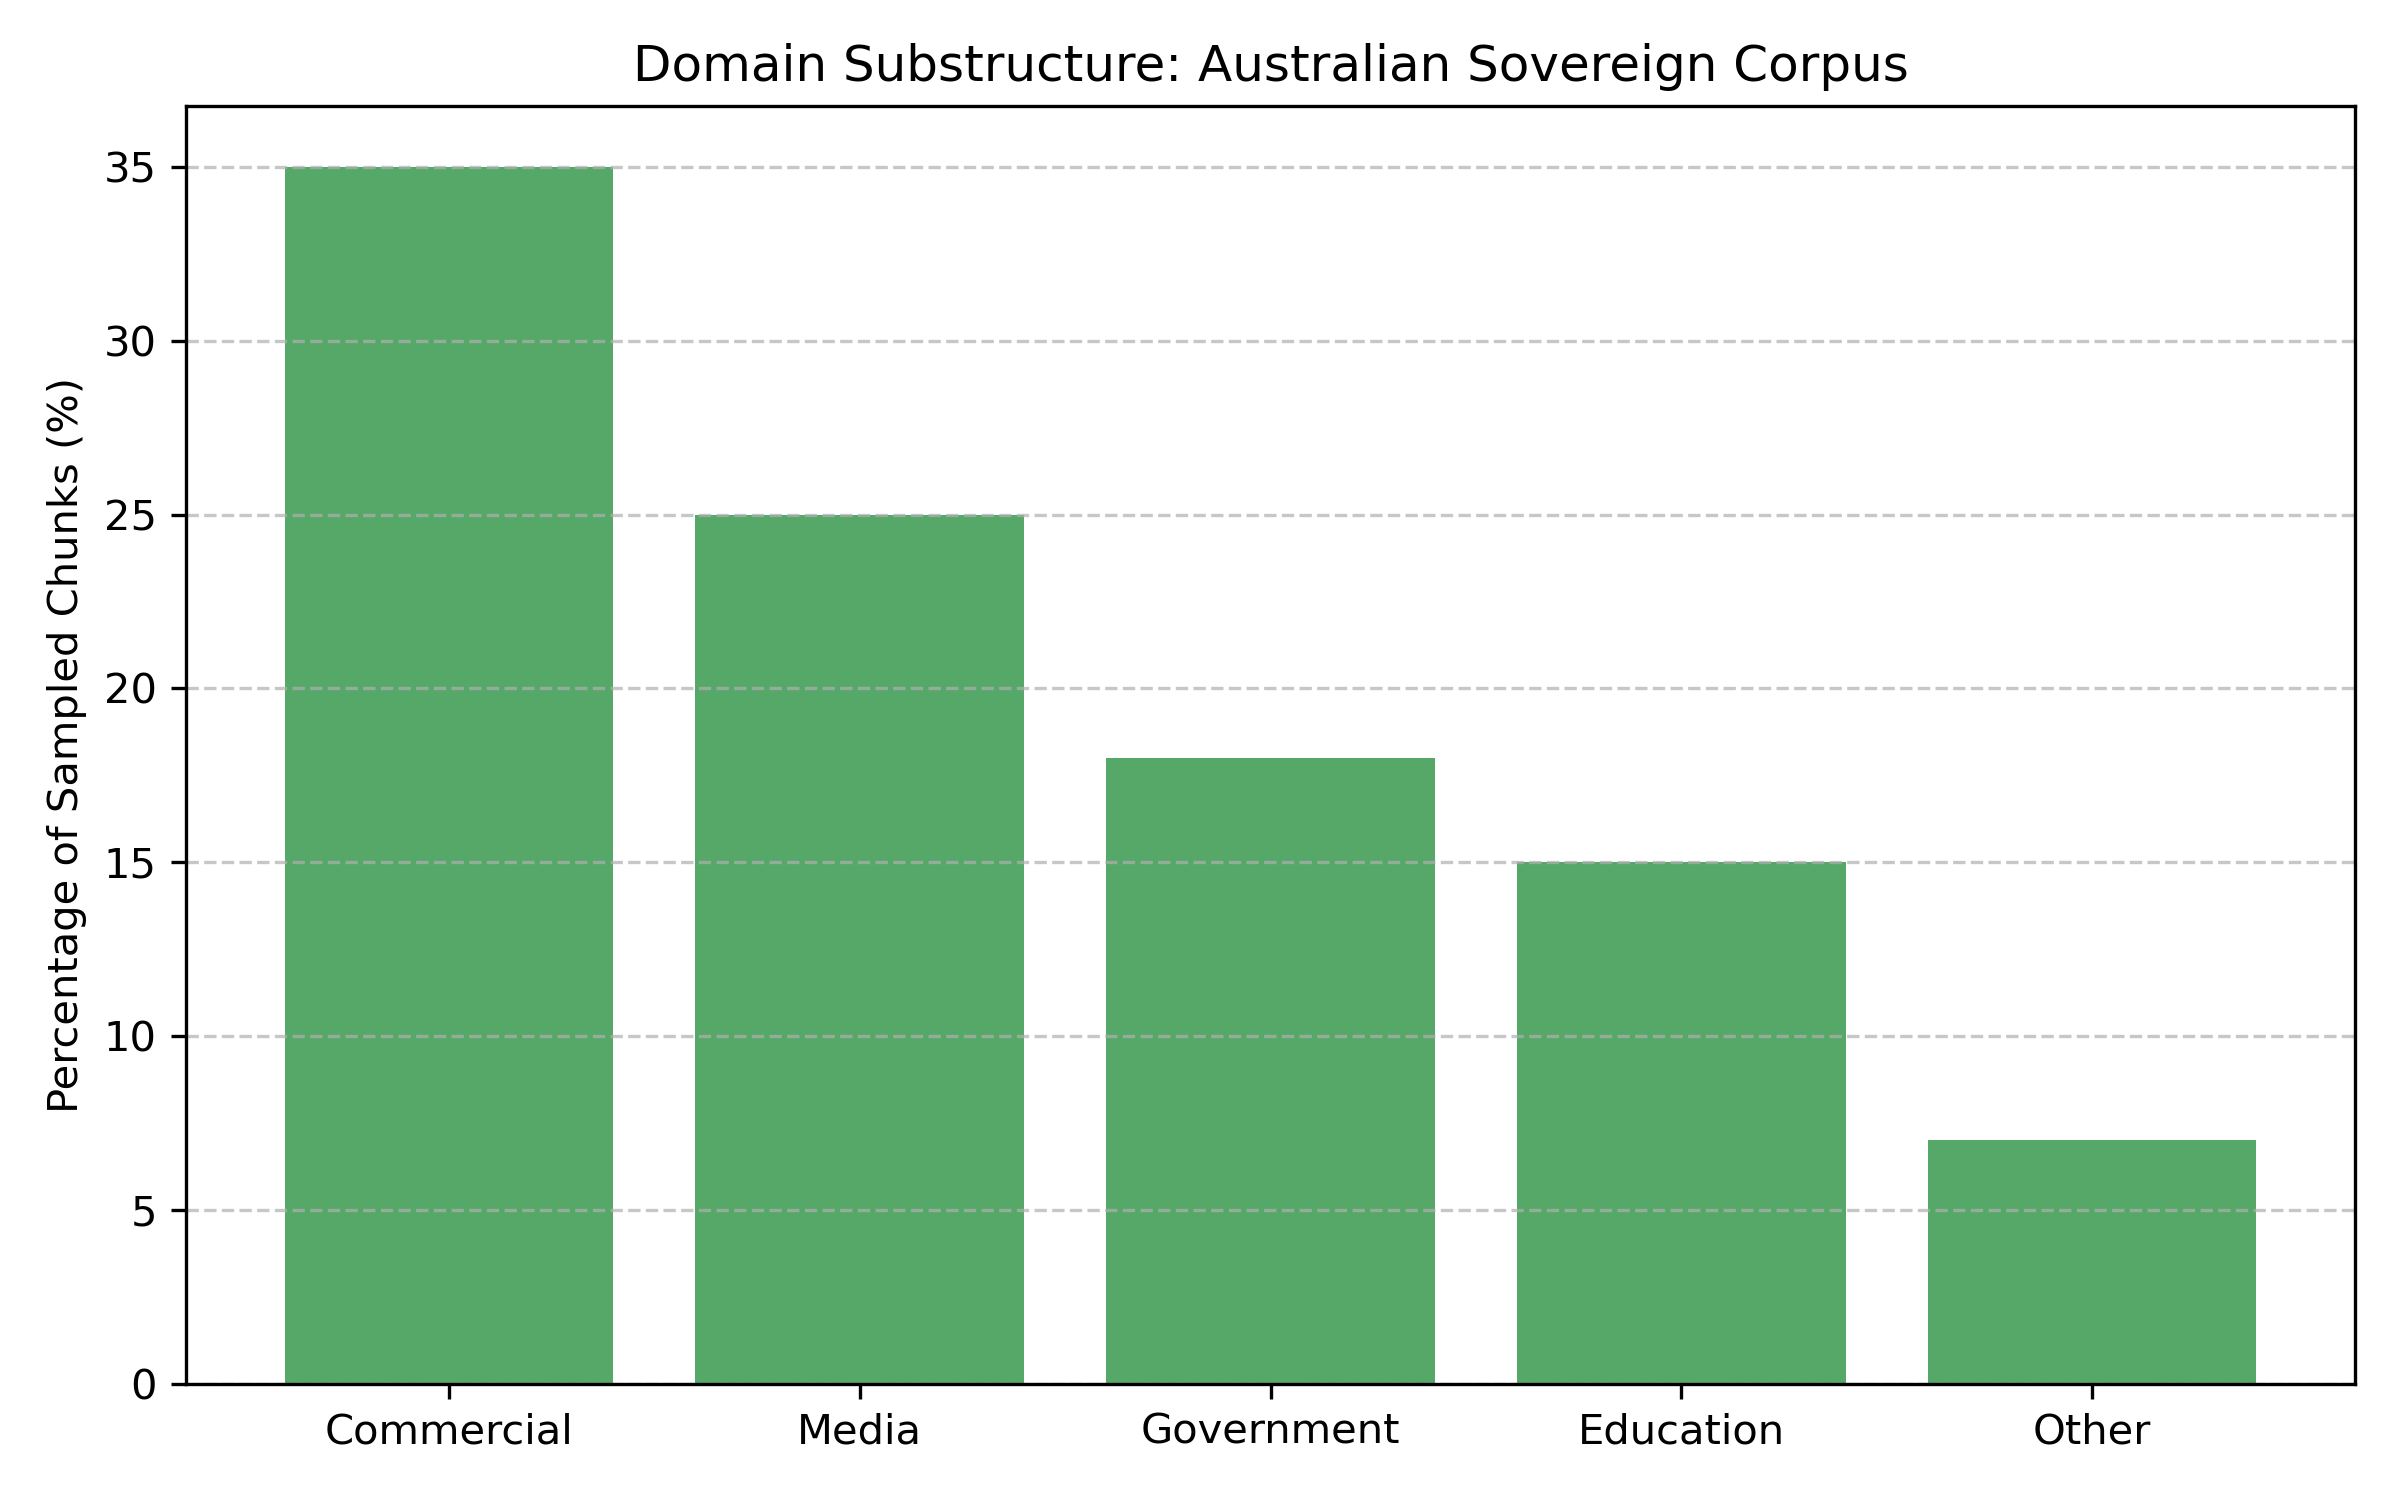
\includegraphics[width=0.85\textwidth]{images/fig5.png}
    \caption{\textbf{Domain Substructure within the Australian Sovereign Corpus.} Fine-grained internal domain breakdown validating that the national dataset can be successfully decomposed into high-confidence sub-corpora for targeted, institutional AI use cases.}
    \label{fig:substructure_au}
\end{figure}

\section{Discussion}

The results of this work demonstrate that it is feasible to construct large-scale, culturally grounded datasets from existing web-scale resources without relying on manual curation or hyperscale infrastructure. By extending established data curation pipelines with structured extraction and refinement stages, it becomes possible to systematically derive region-specific corpora that retain both scale and internal coherence.

A central insight is that cultural grounding emerges from distributional constraints applied during data construction rather than explicit labeling. By restricting the source of the data using structural signals such as ccTLD boundaries, the resulting corpora naturally encode regional language patterns, institutional references, and contextual framing. While these characteristics may be subtle at the document level, they become statistically robust at scale and can be validated through embedding-based and distributional analysis.

This work also highlights a practical limitation in current data pipelines. While high-quality datasets such as FineWeb significantly improve the usability of web-scale data, they do not directly support the extraction of culturally coherent subsets under realistic computational constraints. The approach presented here addresses this gap by enabling downstream dataset construction without requiring repeated large-scale reprocessing of raw web data. This positions the pipeline as an intermediate layer between global data curation and targeted dataset construction.

We acknowledge several limitations. ccTLD extraction is an approximate proxy for geographic origin, and while effective at scale, it does not guarantee perfect alignment. Similarly, embedding-based validation provides a high-level view of dataset structure but does not capture all aspects of cultural nuance. The structural refinement heuristics, while designed to be high-confidence, are also not exhaustive and may allow residual noise to persist.

Despite these limitations, the results indicate that the proposed pipeline provides a practical and scalable framework for constructing sovereign datasets. By making the structure of large-scale web data both visible and controllable, this approach enables more targeted and transparent dataset design. As the demand for regionally aligned AI systems continues to grow, the ability to efficiently construct and validate culturally grounded corpora will become an increasingly important component of AI infrastructure.

\section{Conclusion}

In this work, we introduced a scalable and computationally efficient pipeline for constructing culturally grounded, national-level corpora from web-scale data. By building on the FineWeb processing framework and applying ccTLD extraction paired with targeted structural refinement, we demonstrated the ability to isolate large-scale, region-specific datasets from globally aggregated sources.

Through embedding-based semantic analysis and distributional characterization, we showed that the resulting corpora maintain broad topical coverage while exhibiting coherent internal structure and distinct regional signatures. Cross-country evaluation further confirmed that the pipeline generalizes across multiple jurisdictions, producing datasets that reflect meaningful differences in national content rather than artifacts of the extraction process.

Importantly, the pipeline is designed to operate under realistic computational constraints, enabling web-scale dataset construction without reliance on hyperscale infrastructure. This establishes a practical pathway for research groups and institutions to derive sovereign datasets from existing resources, bridging the gap between global data availability and region-specific data requirements.

While acknowledging the inherent limitations of domain-based proxies and approximate validation methods, this work provides a repeatable and extensible framework for dataset construction. By shifting the focus from large-scale data aggregation to structured data extraction, we lay the groundwork for developing AI systems that are more closely aligned with regional language, context, and institutional knowledge.

As the need for sovereign AI continues to grow, the ability to efficiently construct, analyze, and adapt culturally grounded datasets will become increasingly critical. This pipeline represents a foundational step toward enabling that capability in a scalable and accessible manner.

\section{Data Transparency and Reproducibility}

To ensure methodological reproducibility, we have documented all pipeline artifacts, including the specific domain inclusion lists, structural refinement heuristics, and aggregate token statistics from each processing stage.

While the direct redistribution of the raw, multi-trillion-token extracted dataset is constrained by size and underlying licensing, we are committed to open science and community validation. To that end, we have open-sourced highly curated, \textbf{1-billion-token samples} for each of the four target jurisdictions (Australia, the United Kingdom, Canada, and New Zealand), available via \texttt{Hugging Face}. These subsets consist exclusively of documents that achieved the highest confidence scores within our language and structural quality heuristics.

By sharing these representative national samples alongside our precise architectural artifacts, we provide the research community with the tools necessary to directly evaluate the efficacy of our filtering logic, benchmark cultural grounding, and independently replicate this extraction framework on comparable web-scale sources.

\subsection*{Data Access and Licensing}
The highly curated, \textbf{1-billion-token samples} for each jurisdiction are released openly on \texttt{Hugging Face} under a permissive \texttt{Apache 2.0} license to encourage free community validation and academic fine-tuning. However, the complete, multi-trillion-token extracted corpora are maintained privately. Access to the full, structurally refined datasets is available to non-profit academic research groups upon request, whereas deployment by large commercial organizations requires a commercial licensing agreement. This dual-tier approach recognizes that while the raw underlying web data is public, the systematic structural extraction and targeted refinement pipeline represent significant computational and engineering value.

\subsection*{Dataset Schema}
To facilitate immediate downstream application, the \texttt{Hugging Face} sample releases adhere to a standardized, lightweight schema. Each processed row provides the refined text payload alongside essential provenance and structural metadata. The data is structured as follows:
\begin{itemize}[noitemsep]
    \item \texttt{text}: The fully refined and structurally cleaned document string.
    \item \texttt{url}: The original Common Crawl source URL.
    \item \texttt{cctld}: The extracted top-level domain (e.g., \texttt{.au}).
    \item \texttt{quality\_score}: The upstream \texttt{FineWeb} heuristic score.
    \item \texttt{[Metadata Key]}: [Brief description of additional metadata]
\end{itemize}

\appendix
\section{Before vs.\ After Cleaning Examples}

\textit{[Placeholder for Qualitative Examples]} \\
Table A1 will provide representative text samples demonstrating the efficacy of the structural refinement stage. Examples will contrast text removed due to non-local structural patterns (e.g., conflicting international address formats) against retained content that legitimately discusses international topics from a domestic framing, illustrating the precision of the refinement logic.

\section{Dataset Datasheet}
This datasheet follows the framework proposed by Gebru et al. (2021) to provide transparency and accountability for the sovereign corpora samples released as part of this project.

\subsection{Motivation}
\begin{itemize}[noitemsep]
    \item \textbf{Purpose:} To provide culturally grounded, national-scale datasets for training and evaluating regionally aligned AI systems.
    \item \textbf{Funding:} Southern Cross AI.
\end{itemize}

\subsection{Composition}
\begin{itemize}[noitemsep]
    \item \textbf{Instances:} Web-crawled documents (text-only tokens).
    \item \textbf{Scope:} Australia, United Kingdom, Canada, and New Zealand.
    \item \textbf{Size:} 1 billion tokens per jurisdiction (\texttt{Hugging Face} samples); 1.3 trillion tokens total (full pipeline yield).
\end{itemize}

\subsection{Collection Process}
\begin{itemize}[noitemsep]
    \item \textbf{Source:} Common Crawl (via the FineWeb pipeline).
    \item \textbf{Method:} Domain-based filtering (ccTLD) followed by structural heuristic cleaning.
\end{itemize}

\subsection{Preprocessing and Cleaning}
\begin{itemize}[noitemsep]
    \item \textbf{Steps:} Initial language quality filtering (FineWeb), followed by our secondary structural refinement pass to remove non-local artifacts (e.g., conflicting postal codes and address formats).
\end{itemize}

\subsection{Uses}
\begin{itemize}[noitemsep]
    \item \textbf{Intended Use:} Pre-training foundation models, fine-tuning for regional alignment, and benchmarking cultural knowledge.
    \item \textbf{Restrictions:} Data use is subject to the terms provided by the original source (Common Crawl).
\end{itemize}

\subsection{Distribution}
\begin{itemize}[noitemsep]
    \item \textbf{License:} Compatible with the source data (CC-BY-4.0 / Common Crawl terms).
    \item \textbf{Location:} Available via \texttt{Hugging Face} under the \texttt{JoeyLLM Project} repository.
\end{itemize}

\section*{Acknowledgments}

The author would like to formally acknowledge the contributions of the Master's students from the Australian National University (ANU) TechLauncher program---Nuo Chen, Solomon Inyang, Wen Sun, Xiang Chang, Xingyu Li, and Yingzhe Xu. Their dedicated work in developing, testing, and managing the extraction pipeline repositories was integral to the successful curation of these massive datasets for the \texttt{JoeyLLM} project.

\begin{thebibliography}{99}
\bibitem{commoncrawl} Common Crawl. \url{https://commoncrawl.org/}.
\bibitem{fineweb} Penedo, G., et al. (2024). The FineWeb Dataset: Freshly Phished Tokens. \textit{arXiv preprint arXiv:2406.17557}.
\bibitem{ccnet} Wenzek, G., et al. (2020). CCNet: Extracting High Quality Monolingual Datasets from Web Crawl Data. \textit{LREC}.
\bibitem{gopher} Rae, J. W., et al. (2021). Scaling Language Models: Methods, Analysis \& Insights from Training Gopher. \textit{arXiv preprint arXiv:2112.11446}.
\end{thebibliography}

\end{document}
